
\documentclass[draft]{agujournal2019}
\usepackage{url} %this package should fix any errors with URLs in refs.
\usepackage{lineno}
\usepackage[inline]{trackchanges} %for better track changes. finalnew option will compile document with changes incorporated.
\usepackage{soul}
\usepackage{pdflscape}

\usepackage{xr}
\externaldocument{ms/supp}

\linenumbers

\draftfalse


\journalname{Journal of Advances in Modeling Earth Systems (JAMES)}
\begin{document}
\title{The Community Land Model, version 5.1 \\ One-at-a-time Parameter Perturbation Ensemble}

\authors{D. Kennedy\affil{1,2}, K. Dagon\affil{1}, D.M. Lawrence\affil{1}, R.A. Fisher\affil{3}, B.M. Sanderson\affil{3}, 
N. Collier\affil{4}, F.M. Hoffman\affil{4}, C.D. Koven\affil{5}, E. Kluzek\affil{1}, S. Levis\affil{1}, X. Lu\affil{6}, K.W. Oleson\affil{1}, C.M. Zarakas\affil{7}, Y. Cheng\affil{8}, A.C. Foster\affil{1}, M.D. Fowler\affil{1}, L.R. Hawkins\affil{9}, T. Kavoo\affil{10}, S. Kumar\affil{10}, A.J. Newman\affil{8}, P.J. Lawrence\affil{1}, 
F. Li\affil{11}, D.L. Lombardozzi\affil{1,12}, Y. Luo\affil{12}, J.K. Shuman\affil{13}, A.L.S. Swann\affil{7,14}, S.C. Swenson\affil{1}, G. Tang\affil{1}, W.R. Wieder\affil{1}, and A.W. Wood\affil{1}}

\affiliation{1}{Climate and Global Dynamics Laboratory, NCAR, Boulder, CO, USA}
\affiliation{2}{Earth Research Institute, University of California, Santa Barbara, CA, USA}
\affiliation{3}{CICERO Centre for International Climate and Environmental Research, Oslo, Norway}
\affiliation{4}{Oak Ridge National Laboratory, Oak Ridge, TN, USA}
\affiliation{5}{Climate and Ecosystem Sciences Division, Lawrence Berkeley National Lab, Berkeley, CA, USA}
\affiliation{6}{School of Atmospheric Sciences, Sun Yat-sen University, Guangzhou, Guangdong, China}
\affiliation{7}{Department of Atmospheric Sciences, University of Washington, Seattle, WA, USA}
\affiliation{8}{Research Applications Laboratory, National Center for Atmospheric Research, Boulder, CO, USA}
\affiliation{9}{Department of Earth and Environmental Engineering, Columbia University, New York, NY, USA}
\affiliation{10}{College of Forestry, Wildlife and Environment, Auburn University, AL, USA}
\affiliation{11}{International Center for Climate and Environment Sciences, Institute of Atmospheric Physics, Chinese Academy of Sciences, Beijing, China}
\affiliation{12}{Colorado State University, Fort Collins, CO, USA}
\affiliation{13}{School of Integrative Plant Science, Cornell University, NY, USA}
\affiliation{14}{Earth Science Division, National Aeronautics and Space Administration Ames Research Center, Moffett Field, CA, USA}
\affiliation{15}{Department of Biology, University of Washington, Seattle, WA, USA}
\correspondingauthor{Daniel Kennedy}{djk2120@ucar.edu}

\begin{keypoints}
\item enter point 1 here
\end{keypoints}

\begin{abstract}
\begin{itemize}
\item 211 parameters perturbed
\item featherweight clm configuration, 500x less costly
\item parameter effects can exceed scenario effects
\item large dataset available online providing parameter ranges and effect sizes useful for future studies
\item software infrastructure developed to facilitate routine investigation of parameter sensitivity and uncertainty, as well as automated calibration
\item small number of parameters explains a large fraction of variance 
\item most important parameters can vary regionally and also based on climate forcing

\end{itemize}
\end{abstract}


\section{Introduction}
Water availability, land temperature extremes, fire risk, and crop productivity will all see impacts from climate change, and are among the many processes represented within the terrestrial components of Earth System Models. Understanding how these processes respond to and influence CO$_2$ concentrations is a critical facet of climate change research. Uncertainty in climate model projections varies by domain and generally increases with extended time horizons \cite{koven2022}. Land processes substantially influence climate directly through, for example, evapotranspiration \cite{zarakas2024}, and indirectly through carbon-climate feedbacks.
Making centennial-scale projections of the cumulative terrestrial carbon sink gas been especially challenging, with high uncertainty persisting across model generations \cite{friedlingstein2014,arora2020}, and limited efficacy of emergent constraints. A portion of this uncertainty is irreducible, inherent to the challenge of predicting vegetation dynamics in a novel climate \cite{lovenduski2017}. Still, our expectation is that some of this uncertainty is indeed reducible, if we can more effectively utilize the ongoing expansion of observational data sources from remote sensing, meteorological stations, flux towers, and field campaigns. The capability to efficiently ingest these data and improve simulation performance is especially valuable for actionable science \cite{cheng2023}. However, given increasingly comprehensive land modeling systems, and the wide array of observational products, several technical hurdles exist that hinder effective model development and calibration.

Model inter-comparison projects (MIPs) are a major component of the model development cycle, and have been the primary means by which model projection uncertainty is assessed \cite{henderson-sellers1995,pitman1999,wood1998,schlosser2000,eyring2016,friedlingstein2022}. While MIPs have had tremendous utility in capturing and assessing wide ranges of model assumptions, it can nonetheless be difficult to interpret the differences between models, or even between subsequent versions of the same model, due to the multiplicity of structural and parametric variations \cite{mcneall2016}. In most MIPs, each model is typically allowed only a single parameterization (despite the existence of many plausible parameter sets) due to the high cost of each simulation, e.g. the TRENDY land model intercomparison \cite{sitch2024} or the Coupled Model Intercomparison Project \cite{eyring2016}. Thus, MIPs typically conflate parametric and structural uncertainty, and de-emphasize the consequences of uncertain model calibration in estimates of future land state trajectories. 

Understanding the range of outcomes arising from the many plausible parameter combinations is a critical step in robust uncertainty quantification. 
Parameter sensitivity tests can be used to gauge parametric uncertainty, and
a collection of systematic parameter sensitivity tests across multiple parameters is often termed a Perturbed Parameter Ensemble (PPE, also referred to as Perturbed Physics Ensemble), with examples in the coupled \cite{murphy2004} and land-only contexts \cite{dagon2020,mcneall2024}. 
One important application of PPEs has been assessing uncertainty in climate model projections \cite{murphy2004,sanderson2008,booth2012,hawkins2019,yamazaki2021,peatier2022,tett2022}.
Beyond uncertainty quantification, PPEs also form a basis for automated model calibration through, for example, history matching \cite{williamson2013,williamson2017,hourdin2020,couvreux2021,mcneall2024} or Bayesian methods \cite{cleary2021}.
Several promising avenues for model calibration are in development \cite{pinnington2020,cleary2021,alonso-gonzalez2022}, many of which require the construction of large PPEs \cite{qian2018}.
In a more general sense, PPEs yield a robust knowledge basis for understanding and working with a given climate model. 
This can aid in introducing new users to the model, or to help steer and facilitate model development.

The process of parameter estimation for the complex land models typically embedded within Earth System Models is challenging on account of the intrinsic complexity of the heterogeneous land surface, the diversity and plasticity of plant and microbial life, and the multiplicity of domains that impact the terrestrial biosphere (e.g, hydrology, snow and ice sheets, biogeochemistry, physiology, land management, etc.). The number of model parameters required to represent all the relevant processes is large, and model simulations are relatively expensive, presenting a major barrier to robust objective calibration, model interpretation, and development \cite{fisher2020,dagon2020}.
Thorough assessment of the parametric sensitivity of land models in a manner that is repeatable, open, and integrated with ongoing code development is desirable but challenging \cite{hourdin2017,balaji2022}. It typically requires extensive computational time,  software engineering, and domain-specific expert scientific knowledge.
Our work here tries to alleviate each of these challenges in turn, at least within the context of one land model.
While we are not yet at the point of automated calibration, we present herein several innovations that will serve to make an automated calibration system more technically feasible.

In this project we create a large PPE with the Community Terrestrial Systems Model (CTSM) \cite{lawrence2019}, in the Community Land Model with biogeochemistry configuration (CLM-BGC). We extend the work of \citeA{dagon2020} which utilized a PPE to calibrate a subset of CLM parameters. Here we include a broader suite of parameters and continue to enhance the software tools for parameter perturbation and optimization.
The goal of this project is to systematize the parameter perturbation process within the CTSM modeling framework, and develop the necessary tools and datasets to efficiently test parameter effects across a wide range of land model processes. 
In doing so, we have generated a large PPE, comprising thousands of parameter sensitivity tests.
In this paper we present that dataset, describe how it was produced, and survey some potential applications.
The dataset has already demonstrated utility for diagnosing parameter effects \cite{cheng2023,yan2023a,yan2023b,zarakas2024}, while the software and modeling infrastructure has greatly expanded our capability to generate insights about parameter effects and uncertainties within CTSM/CLM.




\section{Experiment Description}
\label{methods}
\subsection{Model description}
\label{sect:md}
This experiment utilizes the Community Land Model configuration (version 5.1, i.e. CLM5.1) of the Community Terrestrial Systems Model. The model source code and documentation are available online (\url{https://github.com/ESCOMP/CTSM}), as is a full model description \cite{lawrence2019}.

Relative to CLM5.0, version 5.1 includes minor bug fixes, parameter adjustments \cite{birch2021}, and the implementation of biomass heat storage \cite{swenson2019}. The PPE experiment required additional code modifications to enable systematic variation of the full suite of model parameters (many of which were previously `hard-coded', i.e., written directly as numerical values in the model source code). These modifications were incorporated into the main branch of the CTSM codebase for future use (see Open Research Section). We utilized the biogeochemical cycling version of CLM, which includes active carbon and nitrogen cycles. This is as opposed to the satellite phenology mode, which is driven by observed canopy properties and thus has fewer internal feedbacks, and was explored in \citeA{dagon2020}. We used the model in land-only mode driven by reanalysis atmosphere with the crop model turned off.

\subsection{Model spin-up}
\label{sect:mcn}
Model spin-up for the equilibration of carbon and nitrogen pools within biogeochemistry-enabled land models can consume up to 98\% of computational time needed for a simulation \cite{sun2023}. Depending on the evaluation criteria and model configuration, CLM5 requires between 800 and 2000 years (or more) to reach steady-state conditions \cite{lawrence2019}. In the absence of equilibrium, the drift towards steady state can obscure important model dynamics or features \cite{seferian2016}. Because each member of the PPE can have a unique steady state, we performed an independent spin-up for each member.

To manage computational cost we leveraged the Semi-Analytic spin-up mode (SASU) recently implemented within CLM5 \cite{lu2020,liao2023}. This new module utilizes a matrix representation on CLM's biogeochemistry to reduce spin-up time by one order of magnitude \cite{luo2022,liao2023}, and had been previously leveraged for a PPE with the Organizing Carbon and Hydrology in Dynamic Ecosystems (ORCHIDEE) model \cite{huang2018}. Our spin-up protocol featured 20 years in Accelerated Decomposition spin-up mode (see \citeA{lawrence2019} and \citeA{thornton2005} for details), followed by 80 years of SASU, followed by 40 years of Native Dynamic spin-up mode (details on forcing data in Section \ref{sect:exp}). This protocol was designed to achieve sufficiently equilibrated carbon and nitrogen states, while minimizing computational time. This spin-up methodology did not always reach full equilibration of deep soil carbon (beyond 1 meter depth) in very few points at high latitude. Certain inferences about deep soil carbon from this ensemble may therefore subject to uncertainty due to spin-up concerns.

\subsection{Sparse grid}
\label{sect:sg}
Another control on model cost is spatial resolution. Most global CTSM simulations utilize nominal 1$^\circ$ resolution, which equates to about 20,000 land grid cells. In order to manage computational cost, parameter perturbation experiments often use lower resolution, such as 4$^\circ$x5$^\circ$ \cite{dagon2020}. Here, we use a clustering algorithm to achieve an alternative low resolution configuration. The goal is to more strategically distribute grid cells, opting for more grid cells in areas that are especially distinct or variable, and fewer in areas that can be easily approximated based on output elsewhere (e.g. neighboring grid cells). 

Multivariate spatio-temporal clustering (MVSC) has been utilized to extract patterns of climatological significance from climate model output \cite{hoffman2005} and applied to design a representativeness-based sampling network \cite{hoffman2013}. Instead of lowering resolution by coarsening a rectilinear grid, we here used MVSC to strategically remove effectively redundant grid cells.

We used k-means clustering to identify groups of grid cells with similar dynamics based on a 2$^\circ$ transient simulation (1850-2014) using the CTSM-PPE codebase. We selected one representative grid cell from each cluster to stand in for the entire cluster. The representative grid cell is whichever is located nearest the cluster centroid in climate space. The set of representative grid cells comprise a `sparsegrid', which are used in lieu of a `coarse' grid. To recompose mapped output and compute global means, the output from the representative grid cell is substituted for all members of the cluster cohort.

Clustering was based on a subset of 18 CTSM variables (Table \ref{tab:sg}). The MVSC algorithm delineates clusters based on the mean and variability of each variable at each grid cell computed for six 30-year climatology windows (1865-1894, 1895-1924, ... , 1985-2014). Clusters were delineated to equalize the multi-dimensional variance across the user-specified number of groups, $k$. We tested 15 values of $k$, ranging from 10 to 800. Utilizing the ILAMB2.5 benchmarking software \cite{collier2018}, we calculated skill scores to quantify how well each candidate sparsegrid mirrored the full grid output (Supp Figure S1). We opted for a 400-cluster sparsegrid, to balance computational cost against model fidelity. Because our emphasis is on vegetated regions, we masked out Antarctica within the clustering algorithm, whereby we do not provide any output below 60$^\circ$S.

\begin{table}[h]
\caption{Clustering inputs categorized into three groups, with the CTSM variable name in parentheses}
\centering
\begin{tabular}{l c c c c}
 \hline
 Climate variables & Ecosystem state variables &Ecosystem flux variables \\
 \hline
 2m air temperature (TSA) & Leaf area index (TLAI) & Gross primary production (GPP) \\
Atmospheric rain (RAIN) & Ecosystem carbon (TOTECOSYSC) &Heterotrophic respiration (HR) \\
Atmospheric snow (SNOW) &  Ecosystem nitrogen (TOTECOSYSN) &Autotrophic respiration (AR) \\
2m specific humidity (Q2M) & Soil ice (TOTSOILICE) &Net biome production (NBP) \\
Solar radiation (FSDS) & Soil liquid water (TOTSOILLIQ) & Total liquid runoff (QRUNOFF) \\
& Snow cover fraction (FSNO) & Sensible heat  (FSH) \\
&&Latent heat (EFLX\_LH\_TOT ) \\
 \hline
 \end{tabular}
 \label{tab:sg}
 \end{table}

\subsection{Parameter identification and ranges}

Identification of the complete parameter set of a land surface model is in itself a non-trivial exercise, as in practice, many empirical constants are hard-coded and not amenable to systematic perturbation \cite{mendoza2015,cuntz2016}. For the purposes of this activity, we identified a broad set of 211 CLM-BGC parameters, and enabled their modification via the model input files. Several domains were not perturbed, including crops, CH$_4$, VOC, and dust emissions, urban properties, and river flow parameters. The crop model was not utilized as our initial focus is on unmanaged land.
Of the 211 parameters, 145 are scalar-valued, with a single parameter value acting globally. The remaining 66 parameters include a plant functional type (PFT) dimension, with the potential for different parameter values for each unique plant functional type. Not all parameters are currently utilizing this functionality, such as \textit{medlynintercept} where the default value is 100 $\mu$mol H$_2$O for all sixteen of CLM's natural vegetation PFTs.

Given the large parameter space, to conduct an initial analysis of the response of the model to parametric uncertainty, we decided to vary each parameter independently, exploring the impact of low and high values. To define parameter ranges we created an online spreadsheet and solicited domain-area experts to provide a minimum and maximum value for each parameter. In some cases literature values were directly utilized, but in many cases, expert judgment was used. The spreadsheet, with literature references and parameter descriptions is available online and in appendix zqz. In some cases parameters could not or should not be perturbed independently, because they feature inherent co-dependence. In the case of nitrogen fixation costs, we opted to perturb the parameters independently, but also as a group (`KCN'), to enforce a change in overall nitrogen limitation in lieu of switching from one uptake pathway to another. We likewise opted to perturb soil hydraulic parameters directly (e.g. saturated hydraulic conductivity) and also separately via perturbations to the soil texture (percent sand, clay, and silt).

For a small percentage of parameters, the perturbation ranges were severe enough to eradicate a given PFT across all or part of its geographical range (Supp Figure S2). 
In the case that one or more PFTs did not survive a parameter perturbation, we iteratively re-ran the simulation with slightly less extreme parameter values until the PFT survived.
A PFT was classified as surviving in a given gridcell if it achieves an LAI of at least 0.1 m2/m2 at any point during the production portion of the simulation (i.e. post-spinup).
A PFT was classified as surviving for a given parameter perturbation if at least 50\% of the area that
was alive with the default parameters is alive in the perturbed simulation.
For the analyses in this paper, we constrained the ranges of several parameters based on survivability in the low CO$_2$, pre-industrial climate, and control climate ensembles to improve the chances that all PFTs would be able to survive to present-day in a transient 1850 to present-day simulation.
We did not constrain parameter ranges based on future climate, high CO$_2
$, or increased nitrogen deposition.
In total 16 of the 211 parameters had the parameter range constrained to some extent. Original and constrained ranges are available in a supplemental materials spreadsheet.

\subsection{Experimental Design}
\label{sect:exp}
For each of the 211 parameters, we ran 12 simulations, one for each the minimum and maximum parameter values, across six different forcing scenarios.
Each simulation ran for 150 years, with the first 140 for spin-up (as described above in Section \ref{sect:mcn}), followed by a 10-year period for analysis.
It is important to note that these are equilibrium-style simulations, where the land has been allowed to reach steady state conditions relative to the climate forcing. This is achieved by repeating the same 10-year forcing dataset 15 times during the spin-up procedure and production phase of our simulations. As such these simulations are not directly comparable to transient simulations or satellite observations, where present-day vegetation has not yet reached equilibrium with present-day CO$_2$.

 We opted for six different forcing scenarios to understand the intersection of parameter effects with different forcing agents associated with climate change (Table \ref{tab:exps}). The GSWP3v1 reanalysis product (\url{http://hydro.iis.u-tokyo.ac.jp/GSWP3/}) served as our atmospheric forcing, and was the default forcing data for CLM5 \cite{lawrence2019}. We applied climate and CO$_2$ anomalies independently, in order to disentangle their effects on parameter rankings. Future and pre-industrial climate forcing datasets were prepared by adding GSWP3v1 anomalies from 2005-2014 to the corresponding mean climate change signal (see Table \ref{tab:exps}; AF2095 and AF1855). We inferred the mean climate change signal using the CESM2 large ensemble experiment \cite{rodgers2021}, computed as the average of the difference between the period of interest and present day for six atmospheric forcing variables (temperature, humidity, precipitation, wind, longwave and shortwave radiation; see Supp Figure S3 for climatologies). The future climate scenario utilizes the end-of-century climate from the SSP3-7.0, a high-emissions scenario, forcing in line with the existing CESM2 large ensemble \cite{rodgers2021}. Since completing the experiment we uncovered a software bug affecting the AF1855 and AF2095 simulations. Namely that anomalies were not applied to certain coastal gridcells (Supp Fig S4). In all this affected less than 3\% of land area, and did not significantly alter parameter rankings (Supp Fig S5).  


 

\label{sect:exps}
 \begin{table}[h]
 \caption{Forcing Scenarios}
 \centering
 \begin{tabular}{l c c c c}
 \hline
  Name  & Meteorology & CO$_2$ (ppmv) & N addition & Description \\
 \hline
   CTL2010  & 2005-2014 & 367 & - & control experiment\\
   C285        & 2005-2014 & 285 & - & low CO$_2$ \\
   C867        & 2005-2014 & 867 & - & high CO$_2$ \\
   AF1855    & 1851-1860 & 367 & - & pre-industrial climate \\
   AF2095    & 2091-2100 & 367 & - & late century climate (SSP3-7.0) \\
   NDEP      & 2005-2014 & 367 & 5g N m$^{-2}$  y$^{-1}$ & enhanced nitrogen deposition \\
 \hline
 \end{tabular}
 \label{tab:exps}
 \end{table}



\subsection{Biome definitions}
\label{sect:whit}
In addition to analyzing parameter effects on various output variables globally, we were also interested in understanding parameter effects on different biomes.
As such, we categorized each of the 400 sparse grid cells according to their Whittaker biome, which delineates biomes based on average temperature and precipitation \cite{whittaker1970}. 
Biomes were delineated based on the atmospheric forcing temperature and precipitation data averaged across 2005 to 2014 (Supp Figure S6).
Overall there are nine vegetated biomes and an additional ice sheet biome, where no vegetation is present (Supp Figures S7,8).

\section{Results}

Given the very large size of the CLM5-BGC parameter space (Figure \ref{fig:params}), and the relatively expensive computational cost of standard model configurations, a major goal of this project was to develop a fast configuration of CLM5-BGC that would allow for a large number of simulations.
Combining the SASU spinup approach with the sparsegrid formulation (see Section \ref{sect:sg} for details) yielded a configuration approximately 500 times less costly than the 1-degree configuration most often used for CLM simulations (Figure \ref{fig:sims}).
There are 22648, 5666, and 1764 land grid cells in standard 1$^{\circ}$, 2$^{\circ}$, and 4$^{\circ}$x5$^{\circ}$ CLM5 simulations, respectively, as compared to just 400 grid cells in the sparsegrid.
Likewise, whereas previous spin-up methodologies required 1500 years or longer to satisfy equilibrium criteria, the SASU approach enabled by matrix representation yielded satisfactory spin-up efficiency for this experiment within 140 years.

\begin{figure}[h]
\centering
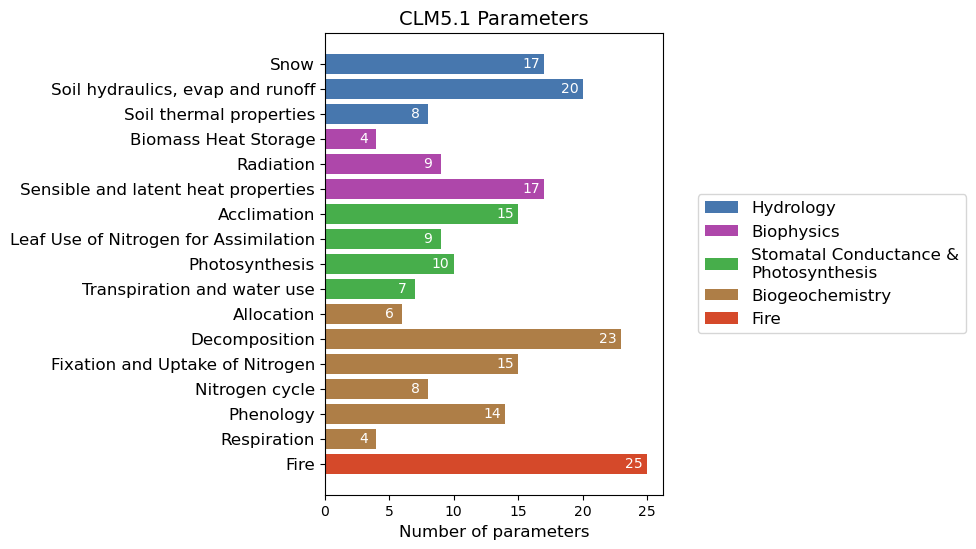
\includegraphics[width=\textwidth]{../figs/main/bar.png}
\caption{211 parameters were perturbed across the various domains of the land model.}
\label{fig:params}
\end{figure}





\begin{figure}[h]
\centering
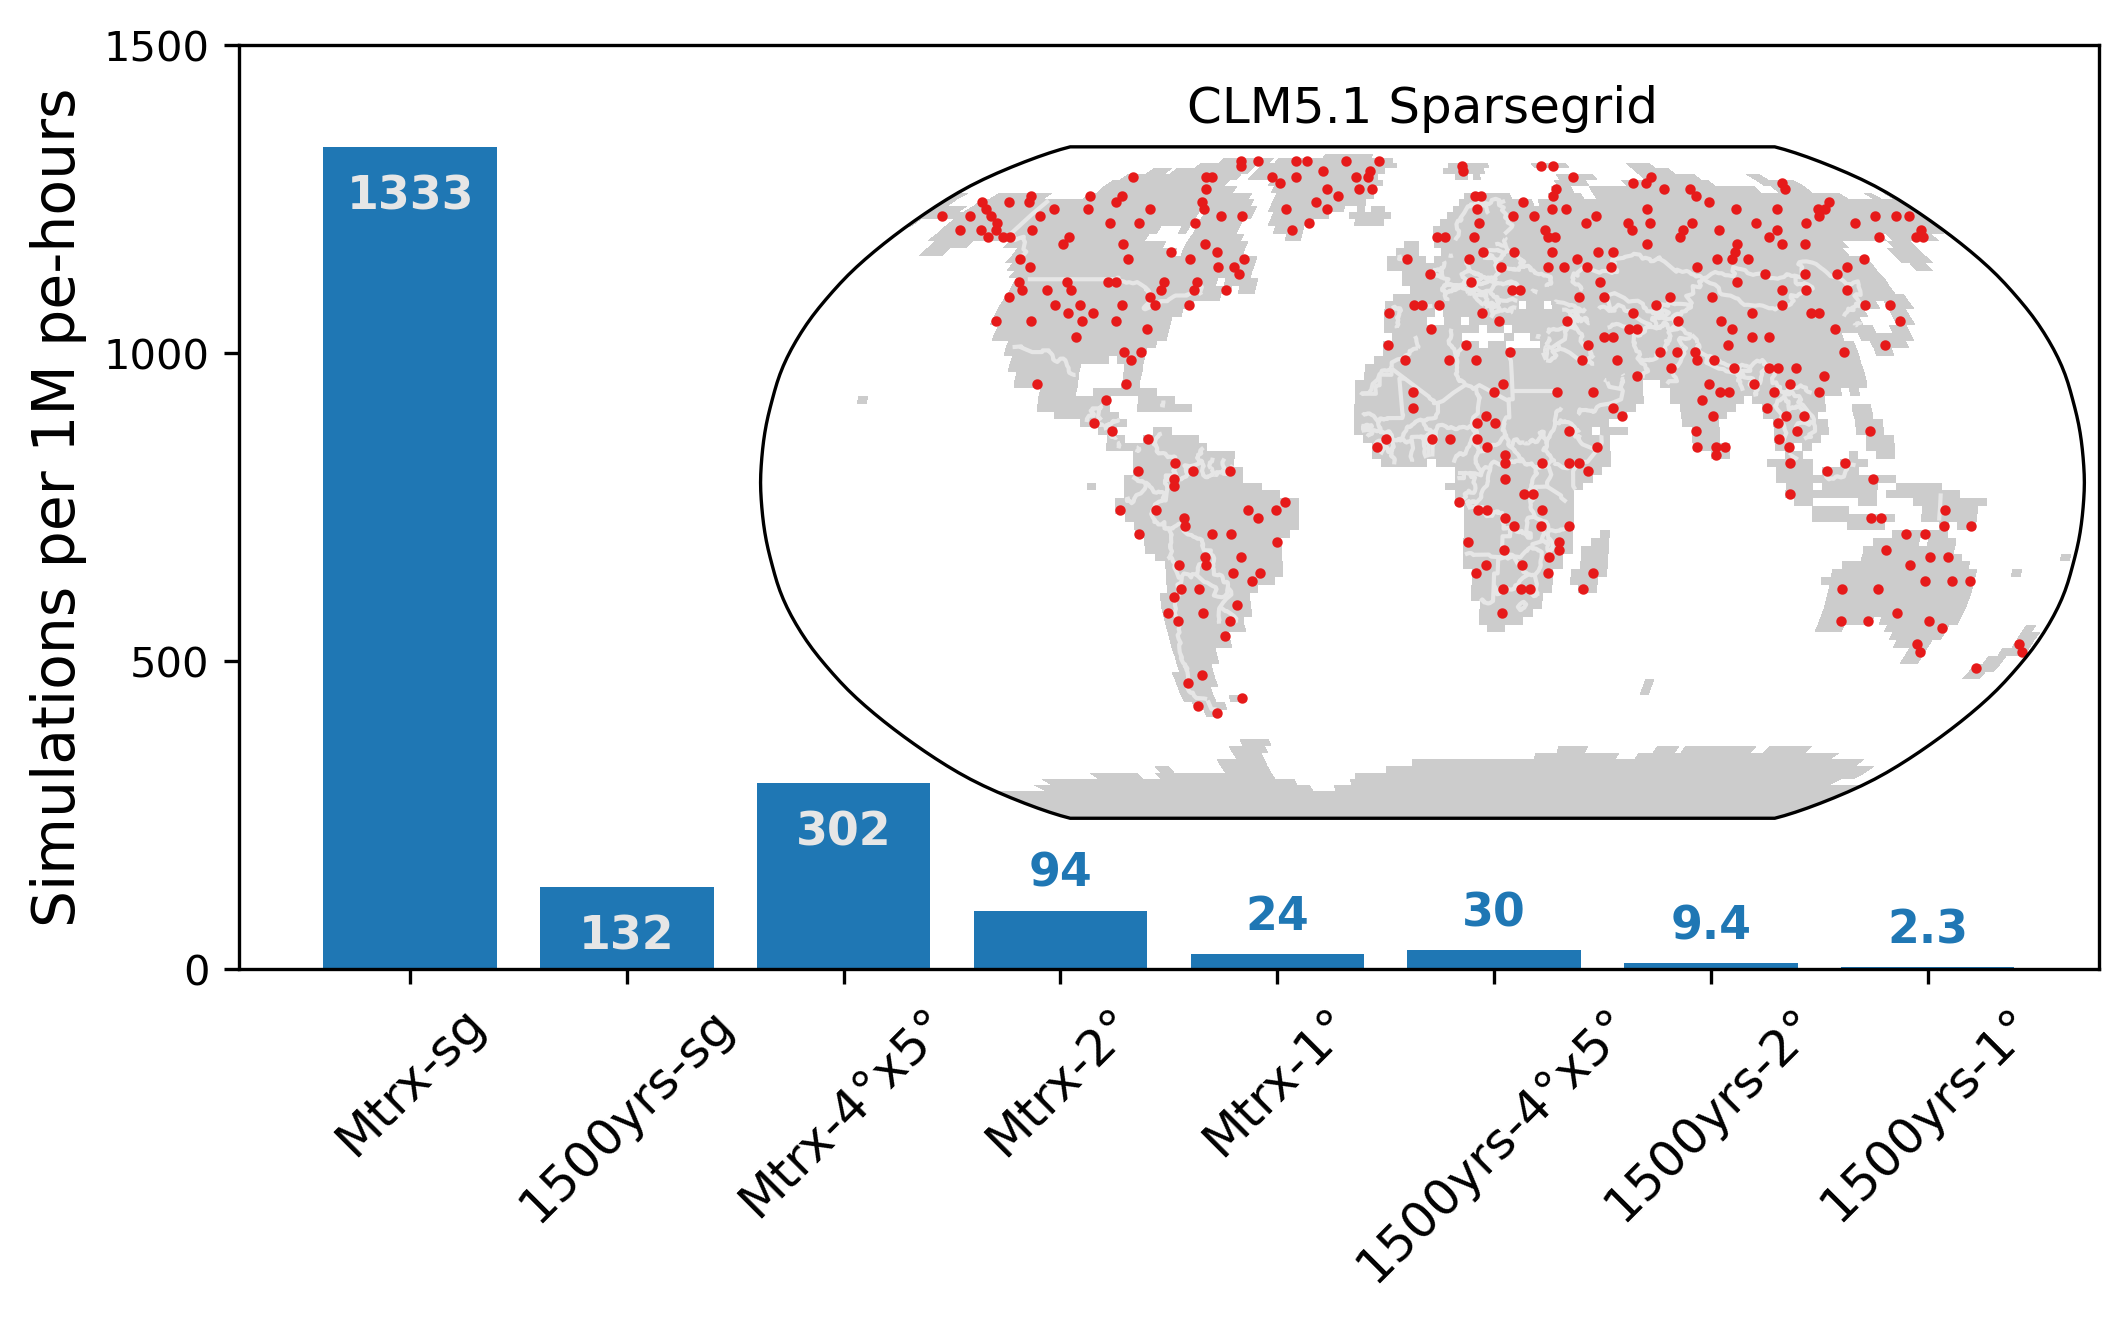
\includegraphics[width=30pc]{../figs/main/sims.png}
\caption{The approximate number of simulations afforded by 1 million core-hours on the Cheyenne supercomputer for a range of CLM configurations. Configurations are labeled according to spin-up procedure (SASU or the standard 1500-year spinup) and horizontal resolution (`sg' signifies sparsegrid). The inset map shows the locations of the 400 sparse grid cells. See Section \ref{methods} for spin-up and sparsegrid details.}
\label{fig:sims}
\end{figure}


Choosing the number of clusters to generate the sparsegrid involved balancing the computational savings against representational fidelity. Given more clusters, the sparsegrid will generally provide a better approximation of output from the full grid. As one example, accurate reconstruction of global photosynthesis could be achieved with a relatively small number of clusters, with R$^2>$0.95 achieved with only 200 clusters (Figure \ref{fig:sg}).
Performance continues to improve with added clusters, but with marginal returns (Supp Figure S2).
We had hoped to see a clear point of diminishing returns across a wide range of variables as we increase the number of clusters. Instead, for most variables, we observe a quick reduction of bias approaching 200 clusters, but after this point, convergence slows and presents some small amplitude oscillations. We chose 400 clusters, because it provides satisfactory performance across a range of important metrics, while affording us sufficient simulations to perform the full experiment within our computational budget.
\begin{figure}[h]
\centering
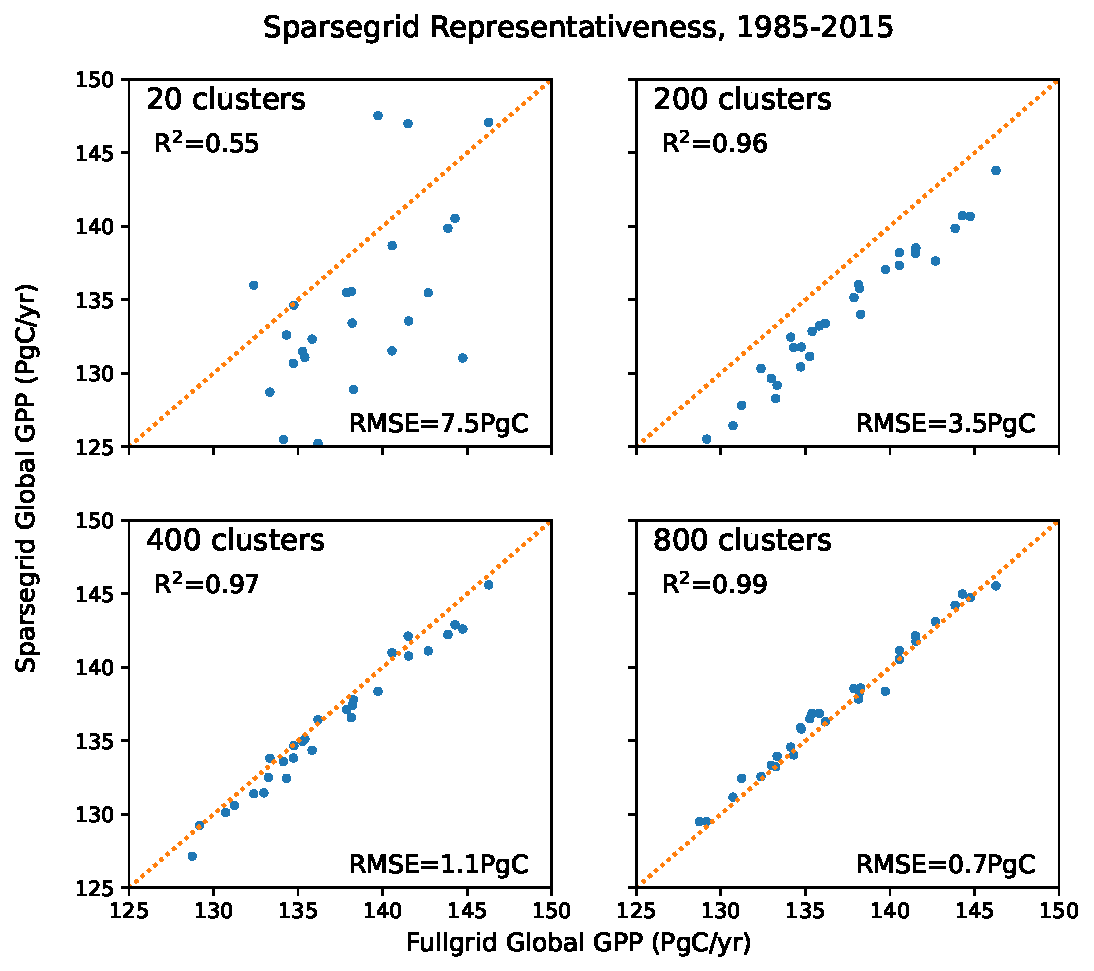
\includegraphics[width=25pc]{../figs/main/sparsegrid_gpp.pdf}
\caption{Sparsegrid vs fullgrid (2$^{\circ}$ resolution) global annual gross primary production (GPP) across the last forty years of a transient CLM5.1 simulation. We opted for 400 clusters to balance computational cost against representativeness.}
\label{fig:sg}
\end{figure}

This model configuration allowed for over 2000 simulations across six forcing scenarios.
Overall, we found substantial impacts of parametric uncertainty on model behavior, in some cases exceeding the magnitude of climate scenario effects (Figure \ref{fig:ranges}). In the control scenario, gross primary productivity (GPP) ranged from 103 to 158 PgC, and net ecosystem productivity (NEP) ranged from 1.7 to 3.8 PgC. NEP was especially variable in the high CO$_2$ scenario, varying from 1.6 to 5.7 PgC. One perturbation, reducing the heat capacity of sand by 20\%, proved destructive in the future climate scenario, resulting in inhospitably hot soil conditions and widespread plant death. A perturbation of $\pm$20\% may exceed the reasonable range for this parameter, but this simulation was instructive for exposing the model's response to hot soils. Carrying out an extensive PPE increases the possibility of exposing unexpected model behavior, including unforeseen tipping points, brittle parameterizations,  and/or bugs.

A small fraction of parameters tends to explain a large amount of the ensemble variance for any given variable or metric (Figure \ref{fig:variance}). For example, just four parameters (maximum leaf wetted fraction, liquid canopy storage, the turbulent transfer coefficient, and leaf characteristic length) explain upwards of 90\% of the canopy evaporation variance across all the forcing scenarios (Supp Fig S3). Conversely, GPP, which is a significantly more complicated process, requires 20 parameters to explain 90\% of the control ensemble variance. In general, most of the parameter perturbations had a relatively small impact on any given output variable. Though this experiment encompasses 211 parameters, no single variable responds to all 211 parameters. In fact, the effective parameter space dimensionality for any given output variable tends to be much smaller than 211. While the principle of land models is that these are all interlinked via complex feedback processes, many parameters nonetheless have impacts that are mostly limited to their own domain. 

\begin{figure}[h]
\centering
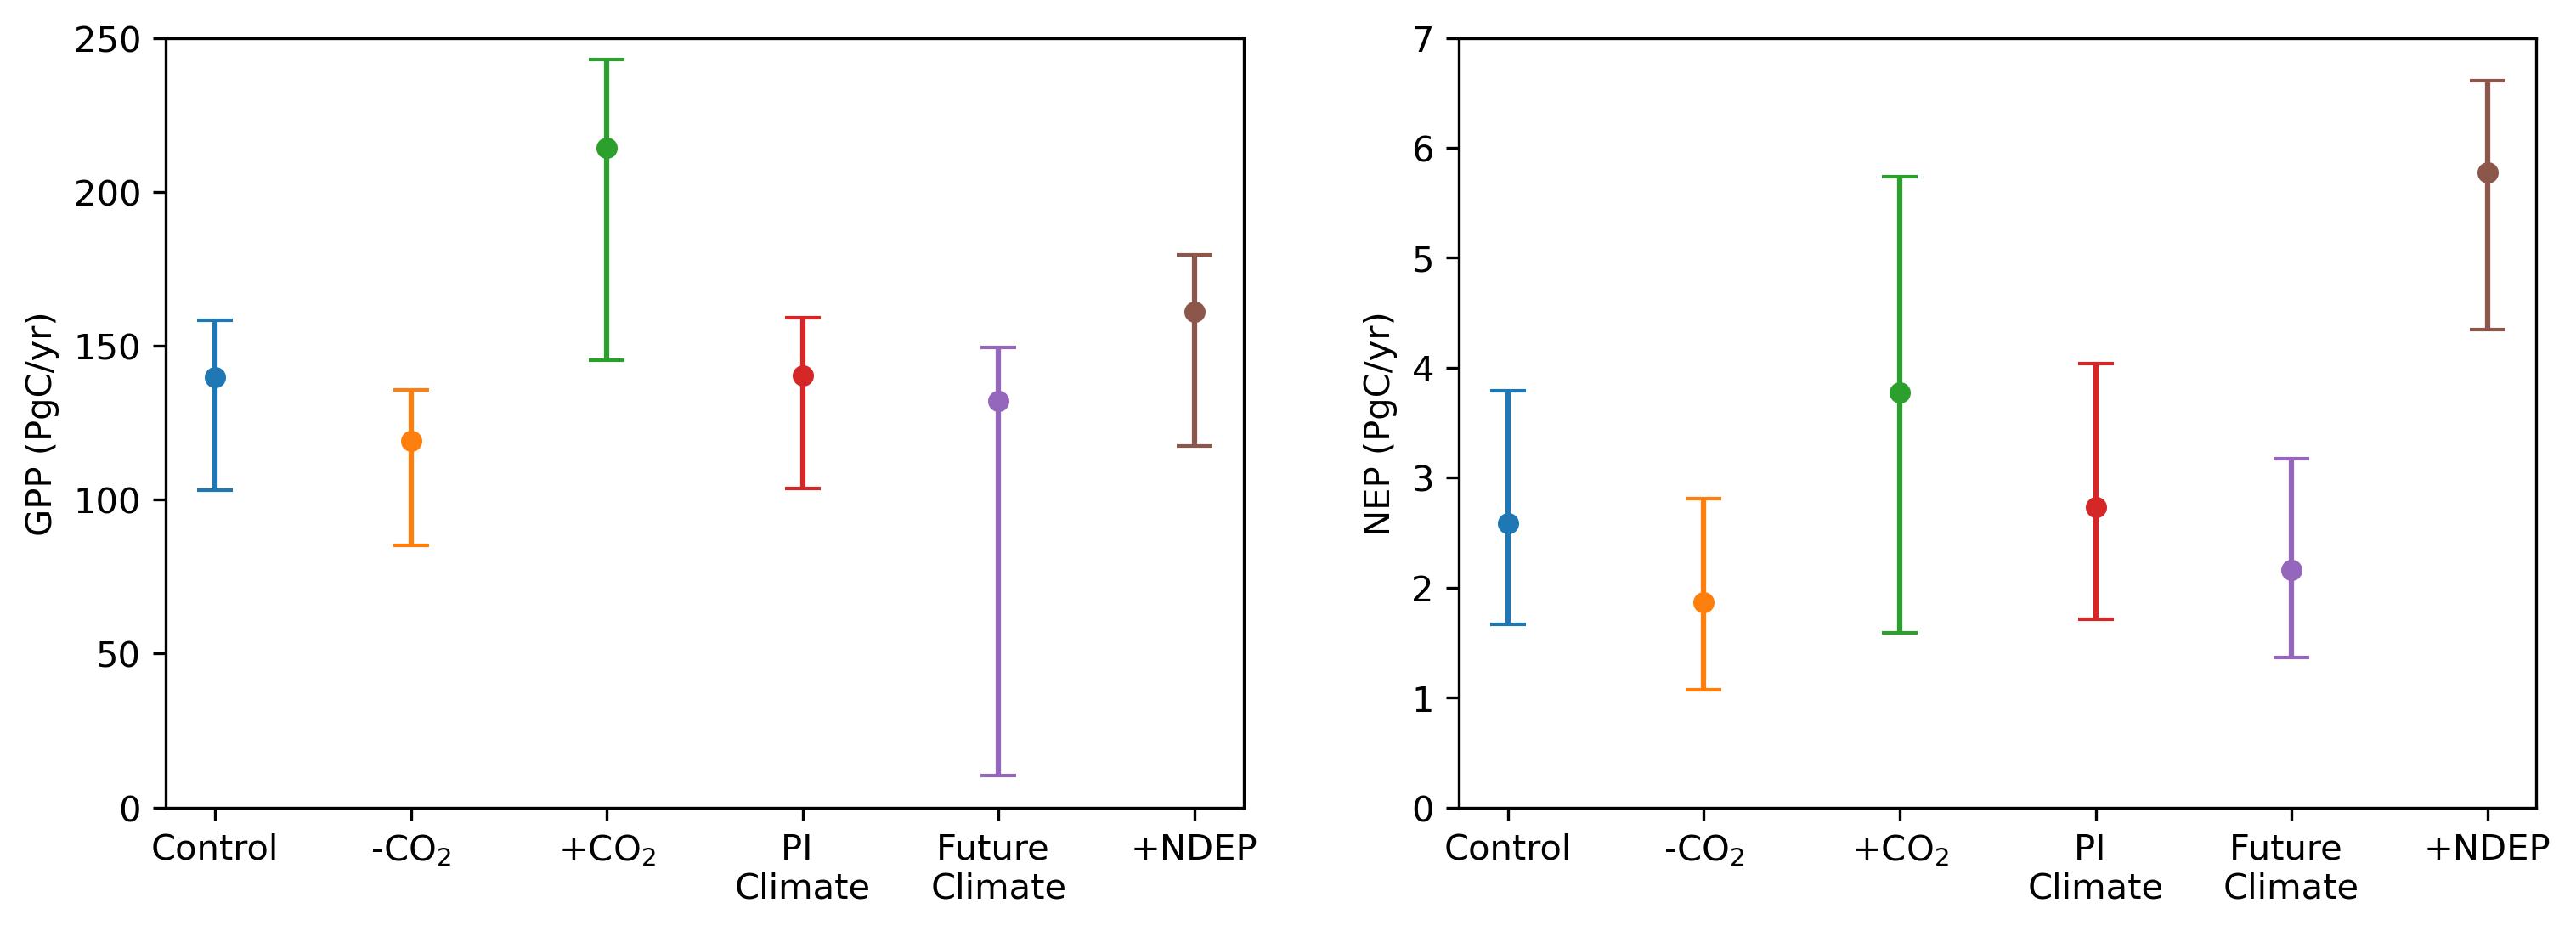
\includegraphics[width=\textwidth]{../figs/ranges.png}
\caption{Global annual gross primary production (GPP) and net ecosystem production (NEP) across six forcing scenarios. Circles mark the CLM5.1 default simulation, and the bars span the ensemble ranges generated by individual parameter perturbations.}
\label{fig:ranges}
\end{figure}

\begin{figure}[h]
\centering
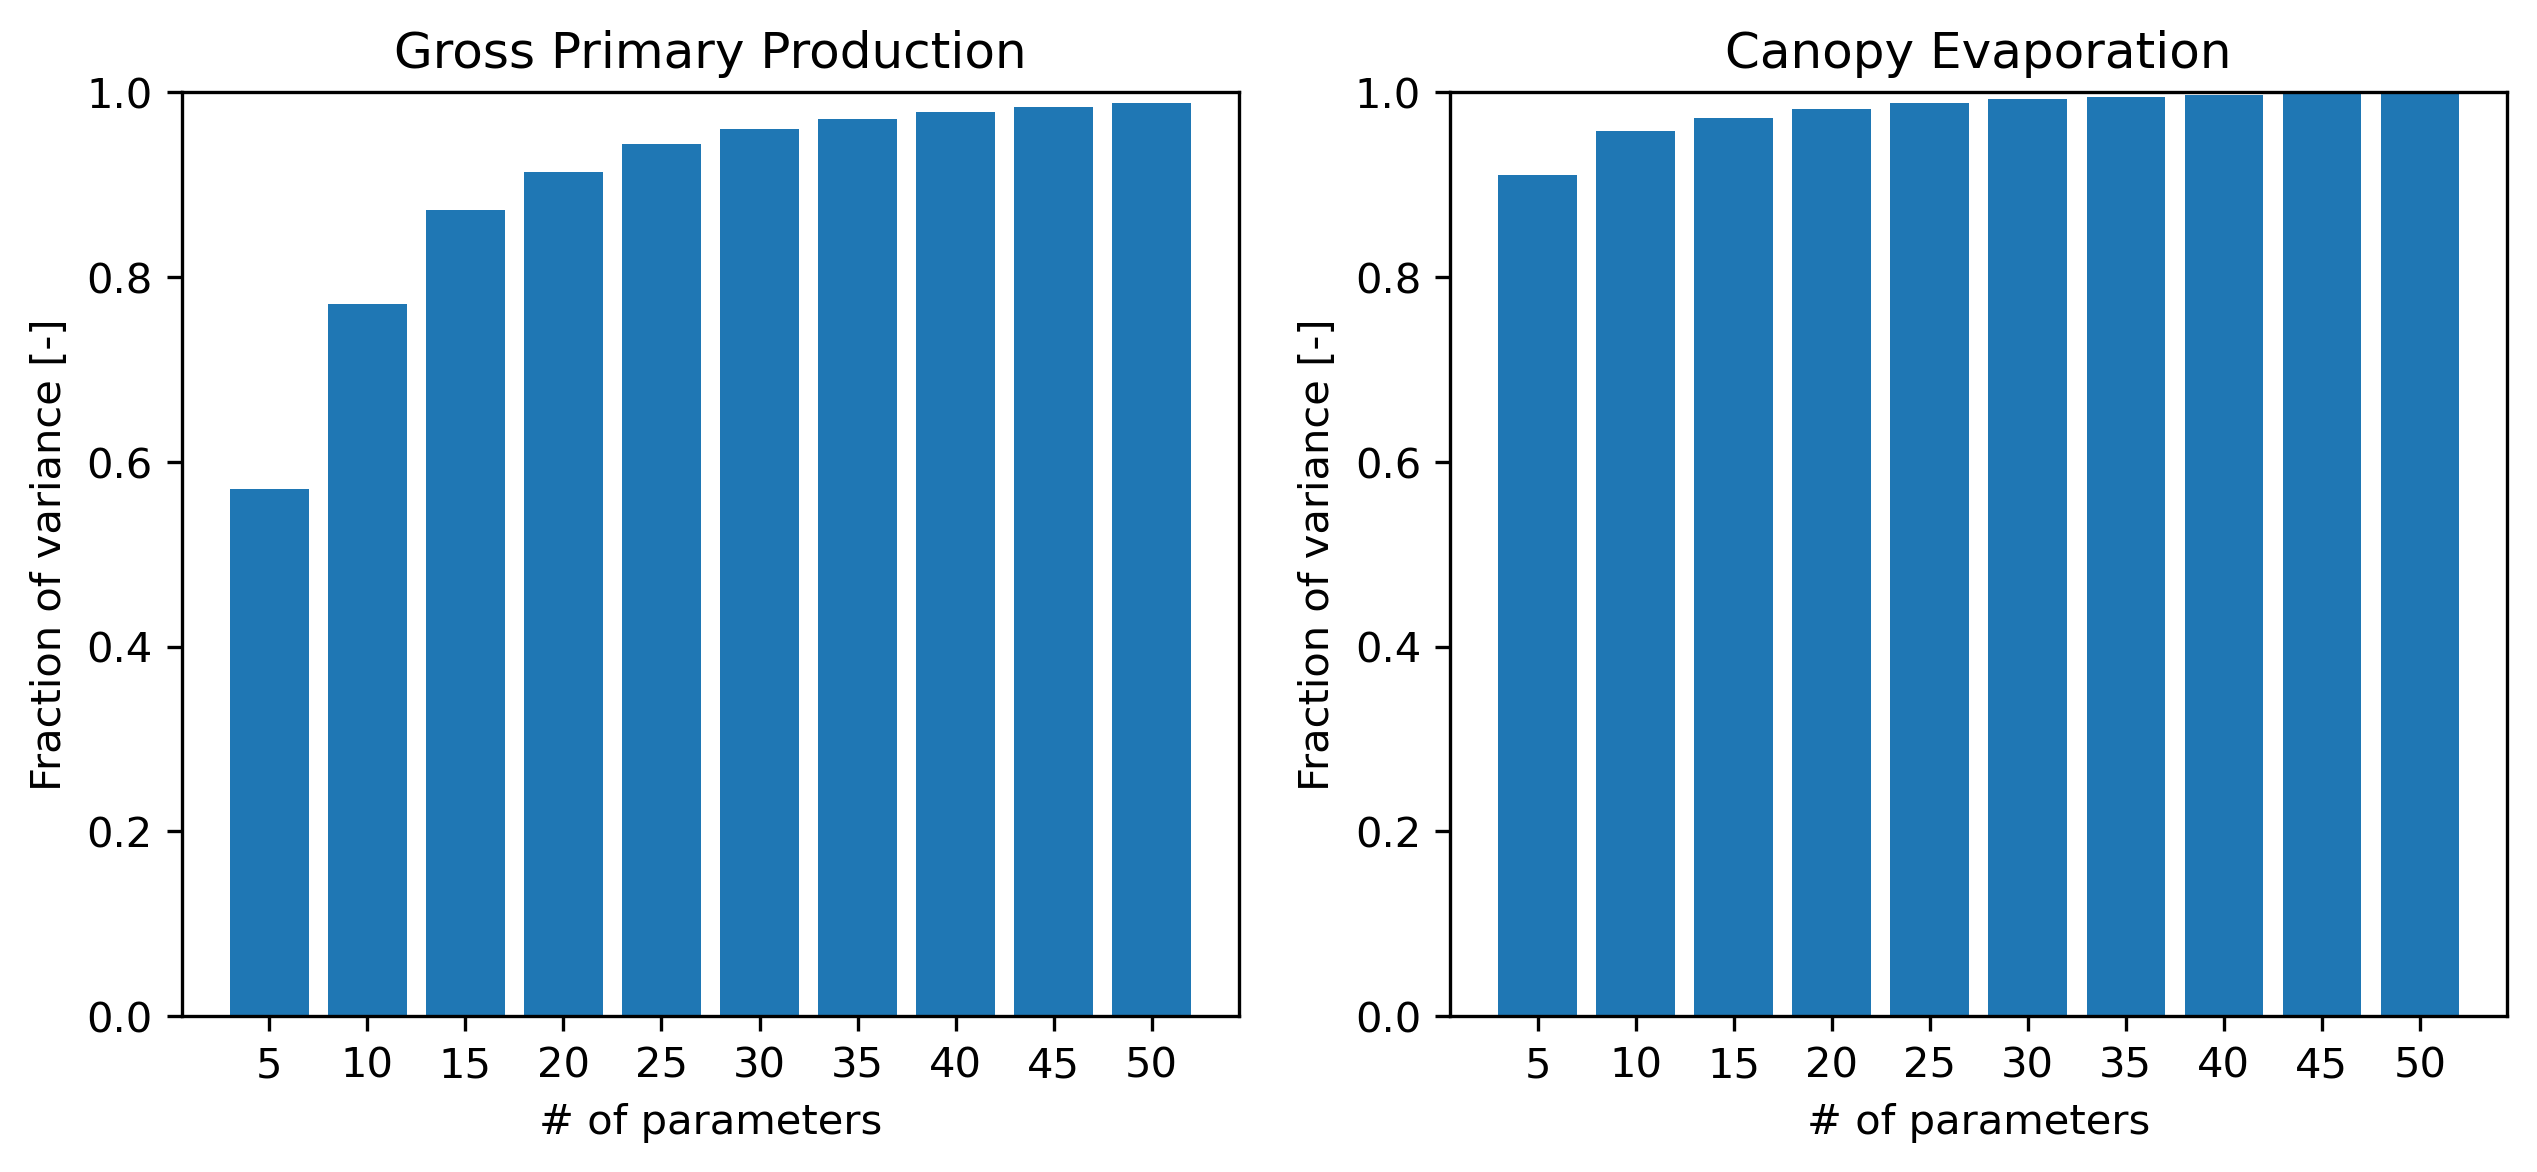
\includegraphics[width=\textwidth]{../figs/variance.png}
\caption{Cumulative fraction of variance explained by the most influential parameters on GPP and canopy evaporation. Approximately 96\% of canopy evaporation variance can be explained by the ten most influential parameters, whereas 30 parameters are required to explain 96\% of GPP variance.}
\label{fig:variance}
\end{figure}

We repeated the full set of parameter perturbations across the six forcing scenarios in Table \ref{tab:exps}. This ensures that we can identify parameters that are important not just under present-day conditions, but also parameters that control the response to forcing (CO2, nitrogen deposition) and climate.
For example, the parameters that control present-day NEP differ  from the parameters that control NEP in the high CO$_2$ scenario (Figure \ref{fig:nep}a,b). NEP increases by approximately 50\% with the increase of CO$_2$ from 367 to 867 ppm when using the CLM5.1 default parameters, but can actually decrease with certain parameter settings (Figure \ref{fig:nep}c). One key parameter is \textit{tpuse\_sf}, which is a scalar perturbation factor influencing the triose phosphate limitations on photosynthesis. Triose phosphate limitation is difficult to quantify and has not been observed to significantly hinder photosynthesis under present-day CO$_2$ concentrations \cite{kumarathunge2019}. In CLM5.1, this parameter is not particularly influential on NEP at 367 ppm (ranked 39, not shown), but is third most influential with high CO$_2$. 

The future climate experiment is 4.3K warmer averaged over our study domain (land-only, Antarctica excluded, Supp Figure S4). This led to an increase in evapotranspiration of 8.8\% relative to the control simulation when using the default CLM5.1 parameters (Figure \ref{fig:nep}f). While the parameters that most strongly affect global average ET in both the control and future climates are generally the same (Figure \ref{fig:nep}d,e), a distinct set of parameters govern the change in ET due to warming (Figure \ref{fig:nep}f). While the control simulation is primarily influenced by hydrology and stomatal conductance parameters, the response of ET to warming is largely controlled by photosynthesis acclimation parameters (i.e. \textit{tpuse\_sf}, \textit{kcha}, \textit{vcmaxha}, \textit{vcmaxhd}, \textit{lmrhd}, and \textit{cpha}). In a coupled ESM, land-atmosphere interactions would modulate these parameter effects, which could dampen parameter effects. While we feel relatively confident identifying influential parameters using land-only simulations, projecting their exact impacts in a coupled framework will require coupled model sensitivity tests.

We repeated parameter ranking analyses in each of nine Whittaker biomes (see Section \ref{sect:whit}). We found that the parameters controlling leaf area index, for example, vary significantly by biome (Figure \ref{fig:lai}). Plant hydraulics parameters were the most important in the tropical rain forest, photosynthetic capacity in the boreal forest, and runoff and soil evaporation in the temperate grassland/desert biome. The most influential parameters for leaf area index globally included parameters that were important in each of these three biomes. 

\begin{figure}[h]
\centering
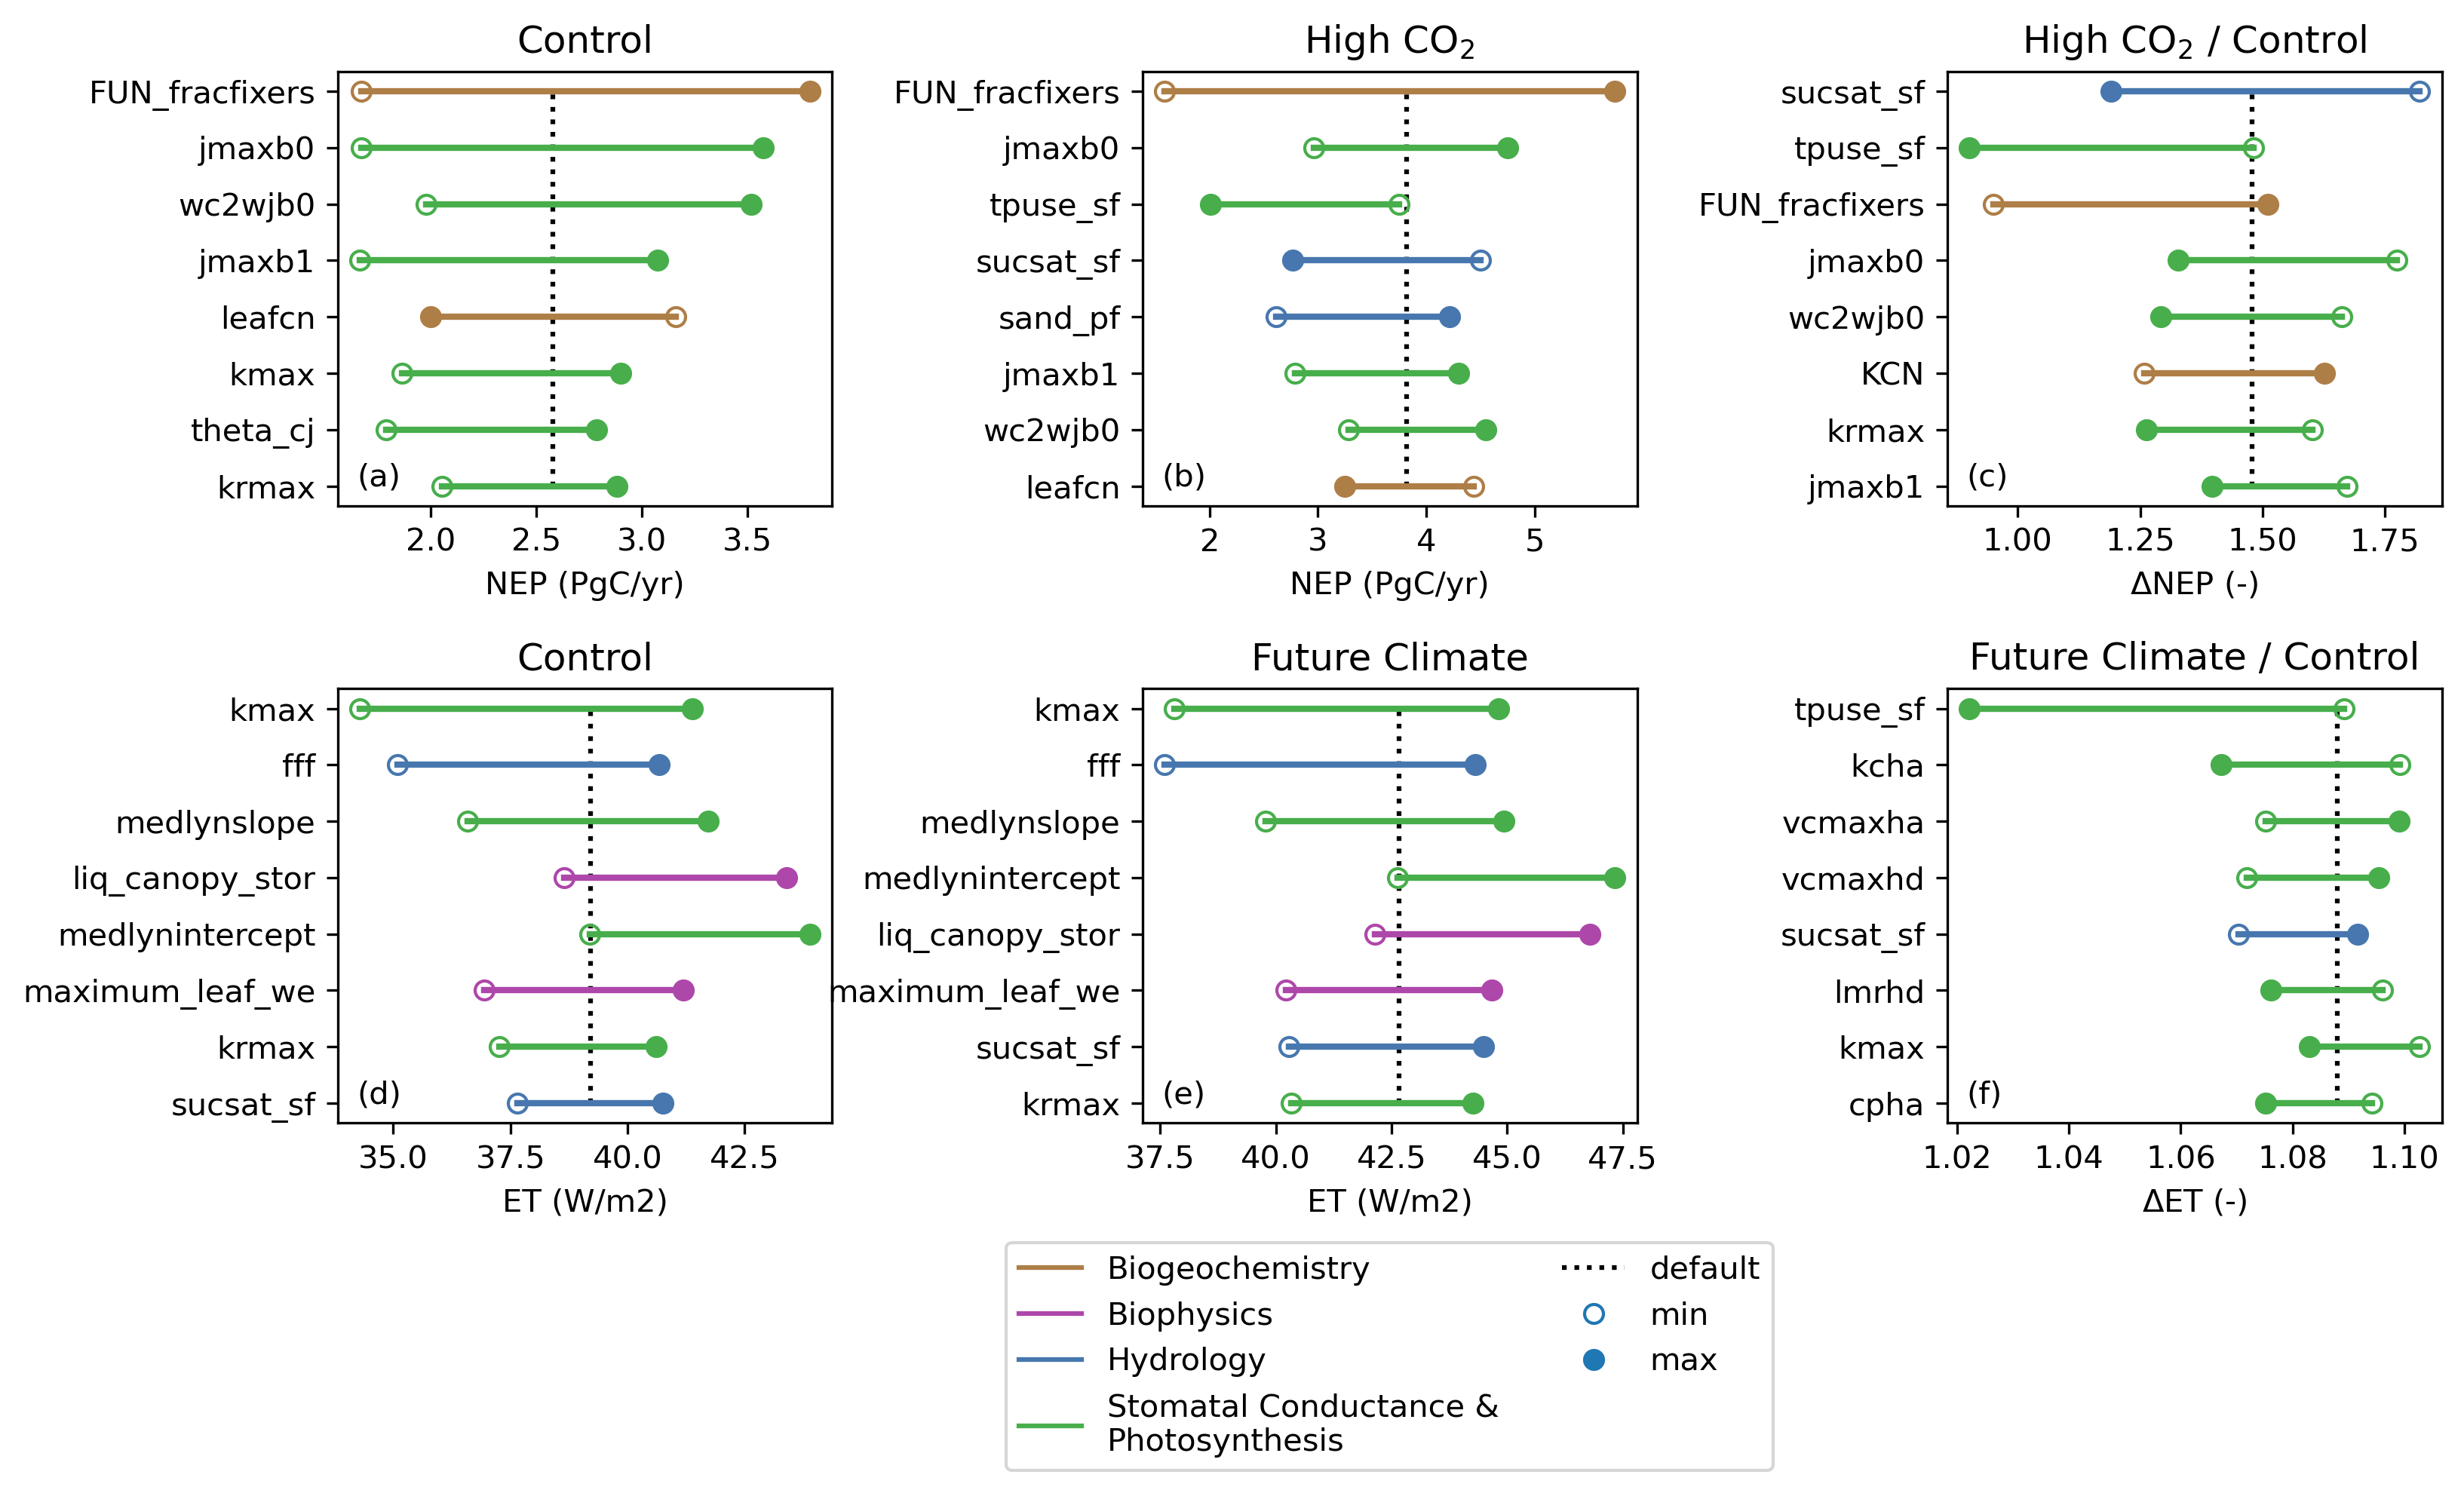
\includegraphics[width=\textwidth]{../figs/main/deltas.png}
\caption{The eight most influential parameters on NEP in the control simulations (a), high CO$_2$ simulations (b), and the relative response to high CO$_2$ (c), as well as on ET in the control simulations (d), future climate simulations (e) and the relative response to future climate (f). The parameters that are most influential on present-day climate (a,d) can differ significantly from the parameters that control the response to forcing perturbations (c,f).}
\label{fig:nep}
\end{figure}


\begin{figure}[h]
\centering
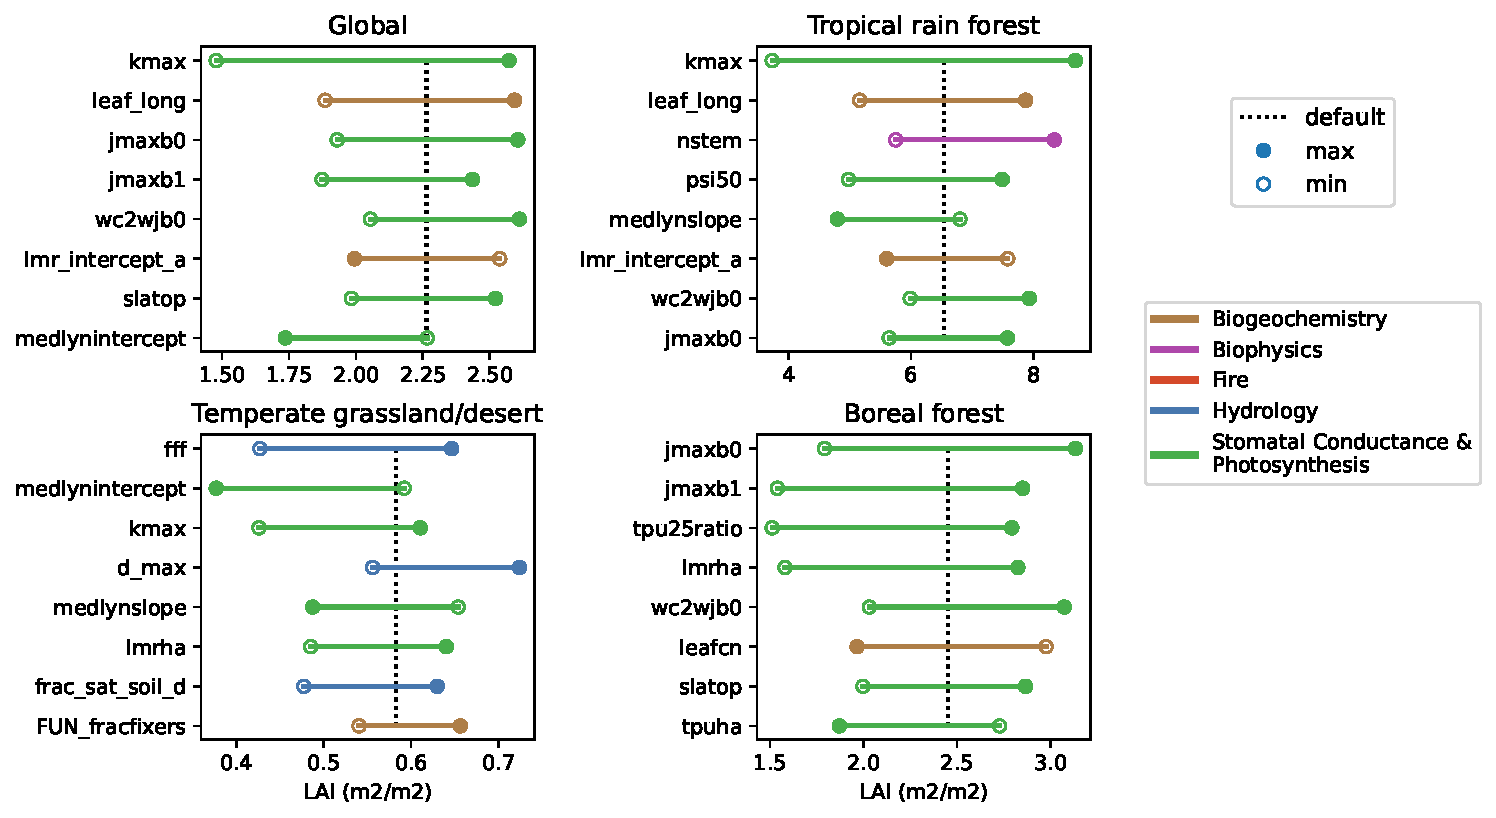
\includegraphics[width=\textwidth]{../figs/lai_biome.pdf}
\caption{The eight most influential parameters on leaf area index within the control ensemble, globally and within three biomes. The solid lines span the range between the two simulations for each parameter, with an open circle indicating the simulation where a parameter is set to its minimum value and a filled circle for its maximum. The lines are color-coded according to scientific domain. The dashed lines indicate the LAI for the simulation with default CLM5.1 parameters. Parameter rankings vary by biome, with the global rankings seeming to reflect contributions from each of these three biomes.}
\label{fig:lai}
\end{figure}

In this paper, we focus primarily on global and biome-level parameter rankings. However it is also possible to inspect the geographic footprint of parameter perturbations by projecting the sparsegrid output to standard lat/lon coordinates (see Section \ref{sect:sg} for details). For example, perturbing the \textit{medlynslope} parameter has a large effect on global runoff, but primarily via its effects in vegetated areas (Figure \ref{fig:map}). 
Because the number of potential variables, parameters, and geographical ranges of interest to the wider CLM community is larger than we can document here,  we provide a tool that can be used to explore an extended diagnostics set which summarises the $>$2TB of output data via approximately 2000 plots (\url{https://webext.cgd.ucar.edu/I2000/PPEn11_OAAT}). The diagnostics website includes ranking plots (as in Figure \ref{fig:lai}) and maps of parameter effects (as in Figure \ref{fig:map}). These plots are repeated across a combination of model output variables and model parameters. Likewise figures are repeated for each of the various forcing scenarios. 




\begin{figure}[h]
\centering
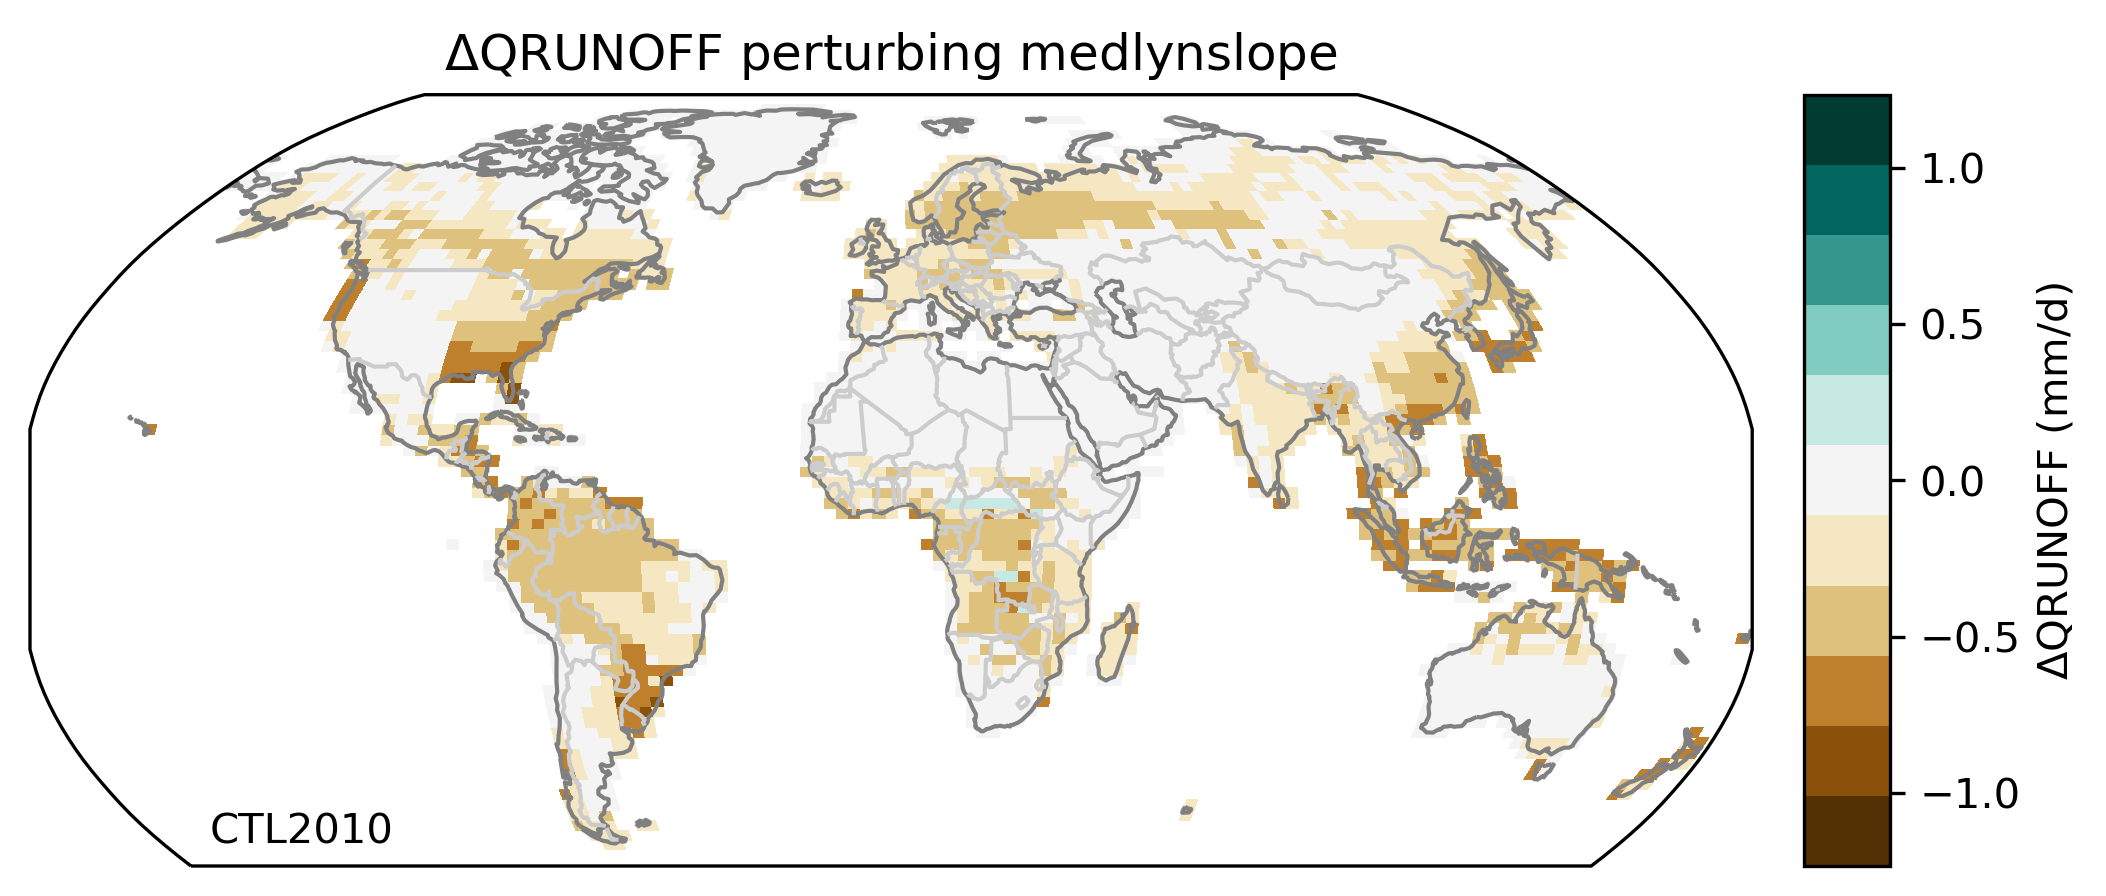
\includegraphics[width=\textwidth]{../figs/QRUNOFFabs_x_medlynslope_CTL2010.png}
\caption{Map of the effect of perturbing medlynslope on runoff within the control ensemble. Increasing medlynslope tends to reduce runoff, but only in regions with sufficient vegetation activity. This is one example of many plots available online (\url{https://webext.cgd.ucar.edu/I2000/PPEn11_OAAT}) in a broader diagnostics set. }
\label{fig:map}
\end{figure}

\section{Discussion}

In this project, we identified and perturbed 211 CLM parameters to create a large one-at-a-time PPE. This ensemble is useful for understanding parametric controls on CLM processes. The software and analysis tools generated to enable and utilize this experiment will greatly reduce the burden of generating future PPEs and parameter sensitivity experiments.

There were several barriers to perturbing the full set of CLM5-BGC parameters. First, many parameters had not been officially identified as such. In such cases, we identified hard-coded values, established an appropriate parameter name, and extracted that parameter to the CLM parameter file for easier manipulation. Although in this experiment we perturbed a large number of parameters (211) across a variety of CLM processes (Figure \ref{fig:params}), this still does not cover the full set of CLM parameters, as some processes were not included, such as crop phenology and management. In carrying out this process of parameter identification, we  likewise unearthed many nuances in  the epistemology of what  `parameters' are in the context of Earth system models. Defining the parameters within a given model structure can be somewhat subjective, such that it would be difficult to collate a comprehensive or definitive set of parameters for a model like CLM.

The second challenge involved defining a perturbation range for each parameter. We solicited expert judgment to set a minimum and maximum reasonable value for each parameter. In some cases, literature values were explicitly used (e.g. for the slope parameter of the stomatal conductance model, `medlynslope', \citeA{lin2015}), but the most common range was $\pm20\%$. It is exceedingly difficult to set parameter ranges that sample comparable probability density, even in a univariate experiment, like this one. The number of parameters is large, with many lacking sufficient empirical backing for robust range evaluation. Defining appropriate ranges for the full suite of land model parameters is a major activity of the scientific subdomains that comprise the land model \cite{kattge2020}. Even with parameters that have an empirical basis, they may behave differently at the coarse climate modeling spatial resolution (zqz), complicating the process of uncertainty quantification. As such, we cannot claim that the parameters are equivalently sampled, whereby parameter effects and parameter rankings could be subject to sampling asymmetries.

The third challenge involved managing computational cost.  Quantifying parameter effects is a necessary prerequisite to automated calibration and uncertainty quantification. Because the parameter space of CLM is quite large and the model response is potentially non-linear, large ensembles are required to adequately resolve response surfaces. With standard CLM configurations, such ensembles would far exceed our computing resources. As such, the computational cost of inferring parameter effects is a major constraint. We were able to reduce ensemble generation computational cost 500x by strategically reducing the number of model grid cells (Figure \ref{fig:sg}) and by leveraging a Semi-Analytic Spin-Up (SASU) offered by the matrix approach to land biogeochemistry models \cite{lu2020,luo2022,liao2023} (see Sections \ref{sect:mcn} and \ref{sect:sg} for details). As long as computational resources remain constrained, designing faster model configurations and efficient sampling strategies will be important for effective model calibration and uncertainty quantification. 

For this experiment we opted for a one-at-a-time perturbation strategy, testing a minimum and maximum value for each parameter. We found that parameter effects could be quite large, in some cases exceeding the effects of our various forcing scenarios (Figure \ref{fig:ranges}). That said, the majority of parameter perturbations had small effects for any specific model variable or metric, such that a majority of simulations were clustered around the default simulation. In the case of canopy evaporation, for example, more than 95\% of the ensemble variance could be explained by the ten most influential parameters (Figure \ref{fig:variance}). This indicates that there may be tractable parameter estimation sub-problems if global calibration of all 211 parameters proves infeasible. 

We opted for six forcing scenarios to identify parameter effects not just in present-day but in response to pre-industrial or future climate conditions. The parameters that were most influential under present-day conditions did not necessarily match the set of parameters controlling the response to future forcing (Figure \ref{fig:nep}). We found that many acclimation parameters, which were not as important for determining present-day evapotranspiration (ET), were among the most influential on the response of ET to future climate. This emphasizes the importance of testing models not only under mean-state conditions, but also under experimentally perturbed conditions under global change analogues \cite{wieder2019}.
Similarly, the parameters controlling leaf area index varied significantly depending on biome (Figure \ref{fig:lai}). 

A one-at-a-time PPE cannot capture parameter interactions, and our min/max sampling protocol precludes diagnosing non-linearities. As such, this dataset will be insufficient for most calibration activities or for estimating overall parametric uncertainty. A primary utility of our dataset is that we can diagnose parameter effects without the uncertainty contributed by an emulator or a regression model. As such, it is easy to diagnose which parameters are most influential on a given process. We have published a large set of ensemble diagnostic plots online, which serves as a valuable enhancement to our model technical documentation. Now, in addition to seeing the definition of a given parameter, and the relevant equations, a model user can easily investigate the magnitude and spatial patterns of its effects (e.g. Figure \ref{fig:map}). This could be useful for investigating obvious model deficiencies, such as regional LAI biases, or to understand potential model responses under different forcing scenarios (e.g. plant survival under low CO2 conditions).  

Our PPE utilizes land-only simulations, with prescribed atmospheric forcing. This is likely to be adequate for estimating many land surface fluxes and pools, in particular of carbon, but could lead to biased estimates of water and energy fluxes, as we know that atmospheric feedbacks to land surface characteristics modify the state of the land surface itself \cite{lague2019}. Additional work is ongoing to extend this work in a coupled model framework to quantify how much, where, and for which processes atmospheric feedbacks are likely to modulate land parameter effects substantially. 

Several spin-off projects have leveraged the work presented here, including some that have already reached publication status \cite{cheng2023,yan2023a,yan2023b}. These projects utilized the output from this ensemble to filter for parameters that influence the relevant study domains and used the parameter ranges collated in Section \ref{sect:exps}. Our project has accelerated parameter exploration work within our collaborator network by providing:

\begin{itemize}
\item Parameter ranges for nearly 200 parameters
\item Purpose-built unstructured grid (sparsegrid)
\item Accelerated spinup procedure
\item Ensemble generation scripting toolchain
\item Parameter sensitivity diagnostics for nearly 200 parameters across 6 forcing scenarios
\end{itemize} 

We have likewise begun a follow-on activity that perturbs a subset of important parameters with the Latin hypercube sampling strategy \cite{mckay2000} to work towards routine model calibration. By investing in the infrastructure that we introduce here, all of our subsequent parameter perturbation experiments have required much less time and effort. We expect to continue to extend our efforts in this domain towards model calibration and uncertainty quantification, as well as repeating the foundational one-at-a-time experiments with subsequent model releases.

\section*{Open Research Section}

The model code for this experiment is contained in a development tag of the CTSM (\url{https://github.com/ESCOMP/CTSM/tree/branch_tags/PPE.n11_ctsm5.1.dev030}).

 (The CTSM component set longname is: \\ \texttt{2000\_DATM\%GSWP3v1\_CLM51\%BGC\_SICE\_SOCN\_SROF\_SGLC\_SWAV\_SIAC\_SESP})

This section MUST contain a statement that describes where the data supporting the conclusions can be obtained. Data cannot be listed as ''Available from authors'' or stored solely in supporting information. Citations to archived data should be included in your reference list. Wiley will publish it as a separate section on the paper’s page. Examples and complete information are here:
https://www.agu.org/Publish with AGU/Publish/Author Resources/Data for Authors


\acknowledgments
This material is based upon work supported by the National Center for Atmospheric Research (NCAR), which is a major facility sponsored by the National Science Foundation under Cooperative Agreement No. 1852977. Computing and data storage resources, including the Cheyenne supercomputer (doi:10.5065/D6RX99HX) were provided by the Climate Simulation Laboratory at NCAR’s Computational and Information Systems Laboratory (CISL). DK is supported via the Drought Task Force IV organized by the NOAA Climate Program Office’s Modeling, Analysis, Predictions, and Projections. FL is supported by the National Key Research and Development Program of China (2022YFE0106500). CDK acknowledges support by the Director, Office of Science, Office of Biological and Environmental Research of the US Department of Energy under contract DE-AC02-05CH11231 through the Regional and Global Model Analysis Program (RUBISCO SFA). RF and BS acknowledge funding by the European Union’s Horizon 2020 (H2020) research and innovation program under Grant Agreement No. 101003536 (ESM2025 – Earth System Models for the Future) and 821003 (4C, Climate-Carbon Interactions in the Coming Century).



\bibliography{refs}

\appendix
\section{Supplementary Figures}


extra text:
Maintaining, improving, and interpreting complex land models benefits from thoughtful investment in software to automate and routinize important components of the development process, e.g. \citeA{collier2018}. 

Will be deleted:
\subsection{Parameters} 
\begin{landscape}
 \begin{table}[h]
 \caption{Some key parameters}
 \centering
 \begin{tabular}{l l c}
 \hline
  Parameter  & Description & Model Domain \\
 \hline
d\_max & Dry surface layer (DSL) parameter & Sensible, latent heat and momentum fluxes \\
frac\_sat\_soil\_dsl\_init & Fraction of saturated soil at which DSL initiates & Sensible, latent heat and momentum fluxes \\
fff & Decay factor for fractional saturated area & Hydrology \\
liq\_canopy\_storage\_scalar & Canopy-storage-of-liquid-water parameter & Hydrology \\
maximum\_leaf\_wetted\_fraction & Maximum leaf wetted fraction & Hydrology \\
medlynintercept & Medlyn intercept of conductance-photosynthesis relationship & Stomatal resistance and photosynthesis \\
medlynslope & Medlyn slope of conductance-photosynthesis relationship & Stomatal resistance and photosynthesis \\
tpu25ratio & Ratio of tpu25top to vcmax25top & Stomatal resistance and photosynthesis \\
jmaxb0 & Baseline proportion of nitrogen allocated for electron transport & Photosynthetic capacity (LUNA) \\
jmaxb1 & Response of electron transport rate to light & Photosynthetic capacity (LUNA) \\
slatop & Specific leaf area at top of canopy & Photosynthetic capacity (LUNA) \\
wc2wjb0 & Baseline ratio of wc:wj & Photosynthetic capacity (LUNA) \\
kmax & Plant segment max conductance & Plant hydraulics \\
krmax & Root segment max conductance & Plant hydraulics \\
psi50 & Water potential at 50\% loss of conductance & Plant hydraulics \\
nstem & Stem number & Biomass heat storage \\
lmr\_intercept\_atkin & Intercept in the calculation of leaf maintenance respiration& Plant respiration \\
froot\_leaf & Allocation parameter: new fine root C per new leaf C & Carbon and nitrogen allocation \\
leafcn & Leaf C:N & Carbon and nitrogen allocation \\
leaf\_long & Leaf longevity & Vegetation phenology and turnover \\
cpha & Activation energy for cp & Acclimation parameters \\
jmaxhd & Deactivation energy for jmax & Acclimation parameters \\
kcha & Activation energy for kc & Acclimation parameters \\
lmrha & Activation energy for lmr & Acclimation parameters \\
lmrhd & Deactivation energy for lmr & Acclimation parameters \\
tpuha & Activation energy for tpu & Acclimation parameters \\
tpuse\_sf & Scale factor for tpu entropy term & Acclimation parameters \\
vcmaxha & Activation energy for vcmax & Acclimation parameters \\
vcmaxhd & Deactivation energy for vcmax & Acclimation parameters \\
 \hline
 \end{tabular}
 \end{table}
\end{landscape}




\end{document}




